\documentclass[a4paper, 12pt]{article}
\usepackage[utf8]{inputenc}
\usepackage[english]{babel} 
\usepackage[margin=3cm]{geometry}
\usepackage[none]{hyphenat}
\usepackage{fancyhdr}
\usepackage{graphicx}
\usepackage{subfigure}
\usepackage{menukeys}
\usepackage{float}
\usepackage{hyperref}
\usepackage{verbatim}
\usepackage{fancyvrb}
\usepackage{fvextra}
\usepackage{listings}
\usepackage{xcolor}
\usepackage{parskip}
\usepackage{csquotes}
\usepackage{ragged2e}
\justifying

\graphicspath{ {../images/} }

\definecolor{codegreen}{rgb}{0,0.6,0}
\definecolor{codegray}{rgb}{0.5,0.5,0.5}
\definecolor{codepurple}{rgb}{0.58,0,0.82}

\lstdefinestyle{mystyle}{
    commentstyle=\color{codegreen},
    keywordstyle=\color{blue},
    numberstyle=\tiny\color{codegray},
    stringstyle=\color{codepurple},
    basicstyle=\ttfamily\footnotesize,
    breakatwhitespace=true,         
    breaklines=true,                 
    captionpos=b,                    
    keepspaces=true,                 
    numbers=left,                    
    numbersep=5pt,                  
    showspaces=false,                
    showstringspaces=false,
    showtabs=false,                  
    tabsize=4,
    postbreak=\mbox{\textcolor{red}{$\hookrightarrow$}\space},
    columns=fullflexible,
}

\lstset{style=mystyle}

\usepackage[backend=biber, style=ieee]{biblatex}
\addbibresource{references.bib}
\nocite{*}

\setlength{\headheight}{15pt}

% setting the format of the page
\pagestyle{fancy}
\fancyhead{}
\fancyfoot{}
\fancyhead[L]{\slshape{\MakeUppercase{Embedded Systems}}}
\fancyhead[R]{\slshape{Davide Sferrazza}}
\fancyfoot[C]{\thepage}

\begin{document}

\begin{titlepage}
    \begin{center}
        \vspace*{1cm}
        \Large\textbf{Università degli Studi di Palermo } \\
        \Large\textbf{Computer Engineering} \\
        \vfill
        \Huge\textbf{Embedded Systems} \\[3mm]
        \Large\textbf{IR Receiver Project \\ on bare-metal Raspberry Pi 4 Model B} \\[1mm]
        \vfill
        By Davide Sferrazza\\
        February 20, 2023
    \end{center}
\end{titlepage}

\tableofcontents
\thispagestyle{empty}
\clearpage

\setcounter{page}{1}

\section{Introduction}
The proposed project consists of using an IR receiver to capture commands sent by a remote controller and displaying them on an LCD display, along with the name of the pressed buttons. \\
This document is organized as follows:
\begin{itemize}
    \item Firstly, I will discuss the hardware used for the implementation, by describing the physical architecture where the software will run and the external necessary harware components that will interact with it;
    \item  Then, I will explain the environment used for project development and how to obtain the parameters needed for the project to function properly;
    \item Lastly, I will illustate how the code was designed and organized.
\end{itemize}

On the last pages you can find the entire code. It is also available online using GitHub (insert link). 

\section{Hardware}
\subsection{Raspberry Pi 4 Model B}
The target of this project is a general-purpose Single-Board Computer (SBC): the Raspberry Pi 4 Model B. 

It is a member of a series of products, which are developed in the United Kingdom by the Raspberry Pi Foundation in association with Broadcom. \\
It  was released in June 2019\cite{Rpi4} and replaced the well-known \textbf{Raspberry Pi 3 Model B} and \textbf{Raspberry Pi 3 Model B+}.

\begin{figure}[h]
    \centering
    \subfigure[Hardware]{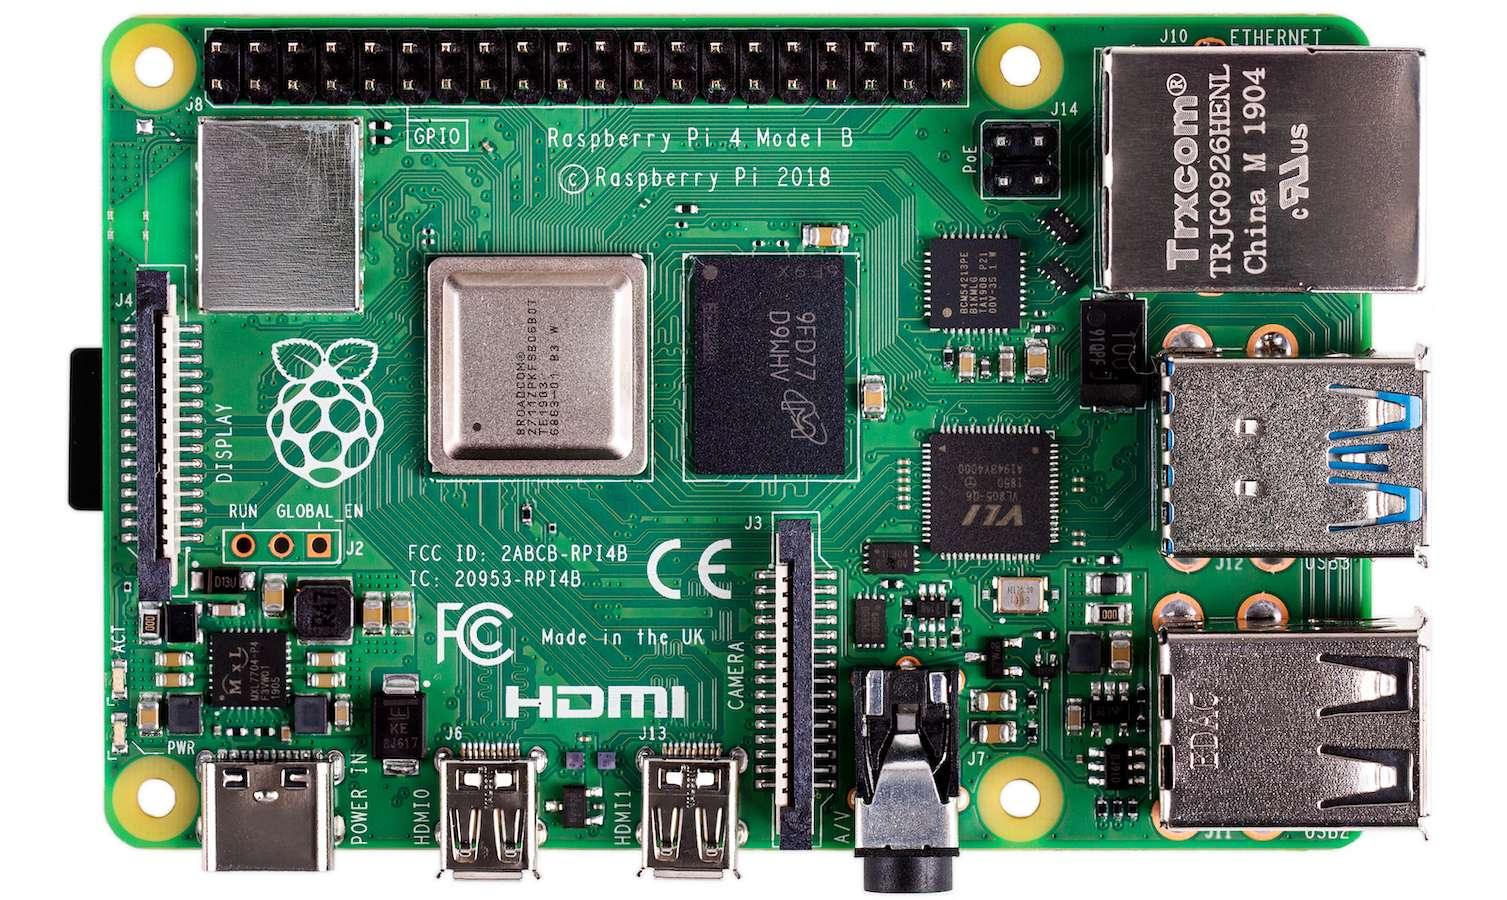
\includegraphics[width=7cm]{pi4}} 
    \subfigure[40-pin Header]{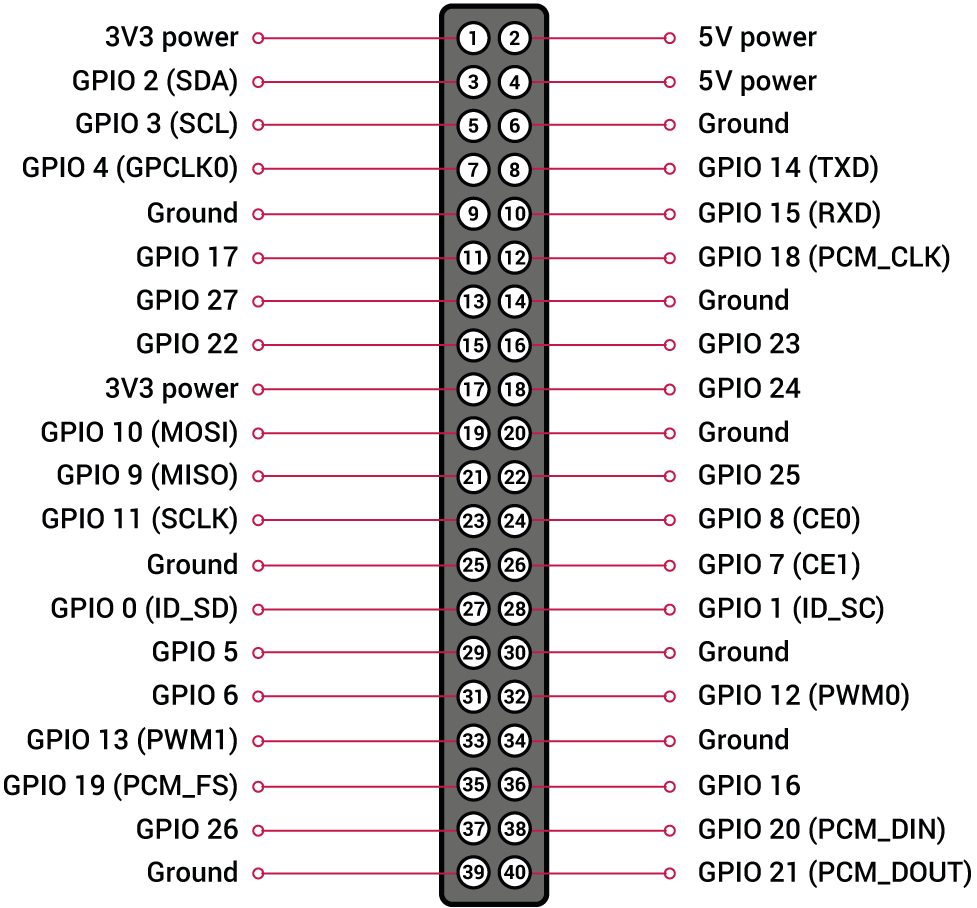
\includegraphics[width=5.52cm]{GPIO-Pinout-Diagram-2}} 
    \caption{Raspberry Pi 4 Model B}
\end{figure}

It is built with the following specifications\cite{SpecsRpi4}:
\begin{itemize}
    \item Broadcom BCM2711, Quad core Cortex-A72 (ARM v8) 64-bit SoC @ 1.5GHz;
    \item 1GB, 2GB, 4GB or 8GB LPDDR4-3200 SDRAM (depending on model);
    \item 2.4 GHz and 5.0 GHz IEEE 802.11ac wireless, Bluetooth 5.0, BLE;
    \item Gigabit Ethernet;
    \item 2 USB 3.0 ports; 2 USB 2.0 ports;
    \item Raspberry Pi standard 40 pin GPIO header (fully backwards compatible with previous boards);
    \item 2 × micro-HDMI ports (up to 4kp60 supported);
    \item 2-lane MIPI DSI display port;
    \item 2-lane MIPI CSI camera port;
    \item 4-pole stereo audio and composite video port;
    \item H.265 (4kp60 decode);
    \item H264 (1080p60 decode, 1080p30 encode);
    \item OpenGL ES 3.1, Vulkan 1.0;
    \item Micro-SD card slot for loading operating system and data storage;
    \item 5V DC via USB-C connector (minimum 3A*);
    \item 5V DC via GPIO header (minimum 3A*);
    \item Power over Ethernet (PoE) enabled (requires separate PoE HAT);
    \item Operating temperature: 0 – 50 degrees C ambient.
\end{itemize}
The model I used comes with 4GB of RAM.

\subsection{FTDI Adapter FT232RL}
Since modern computers do not expose serial ports to program the SBC, a UART (Universal Asynchronous Receiver-Transmitter) serial adapter is required. 

\begin{figure}[h]
    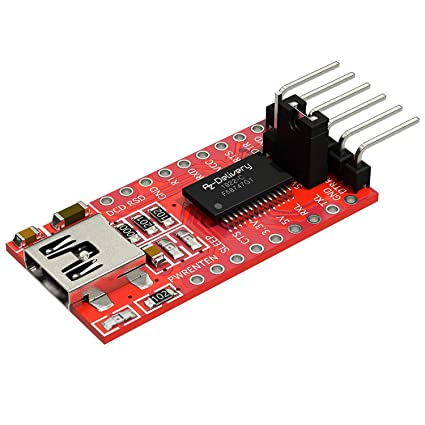
\includegraphics[width=6cm]{FT232-AZ}
    \centering
    \caption{FTDI Adapter FT232RL from Mini-USB to TTL}
\end{figure}

I adopted the Mini-USB to TTL serial adapter provided by AZ-Delivery\cite{FTDIAdapter}. \\
To avoid voltage problems power is supplied from the terminal used to develop the project and is shared between the Pi 4 and the FT232RL. \\ 
The connection is made in the following way:
\begin{itemize}
    \item FT232RL RX pin is connected to GPIO 14 (TXD);
    \item FT232RL TX pin is connected to GPIO 15 (RXD);
    \item FT232RL GND pin is connected to the GND of the Pi 4.
\end{itemize}

\subsection{KY-022 Infrared receiver module}

IR detectors\cite{ELEGOO} are little microchips with a photocell that are tuned to listen to infrared light. They are almost always used for remote control detection - every TV and DVD player has one of these in the front to listen for the IR signal from the clicker. Inside the remote control is a matching IR LED, which emits IR pulses to tell the TV to turn on, off or change channels. IR light is not visible to the human eye, which means it takes a little more work to test a setup.

\begin{figure}[h]
    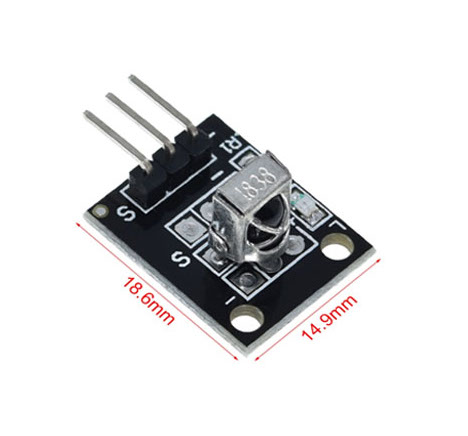
\includegraphics[width=8cm]{ir_module}
    \centering
    \caption{KY-022}
\end{figure}

The module is able to detect frequencies ranging from about 35 KHz to 41 KHz, but the peak frequency detection is at 38 KHz.

The IR receiver comes with 3 pins: the digital signal output pin (S) used to read the value of infrared light, the power pin (+) and the ground pin (-).

When it detects a 38KHz IR signal, the output is low. When it detects nothing, the output is high. \\
It requires a supply voltage in $[2.7, \, 5.5]$V, so it is powered by the Pi 4 using one of the 3V3 pins. Its GND pin is connected to the GND of the Pi 4.

Its output pin is connected to GPIO 25.

\subsection{Samsung AA59-00584A}

The TV remote controller I used is produced by Samsung.

\begin{figure}[h]
    \centering
    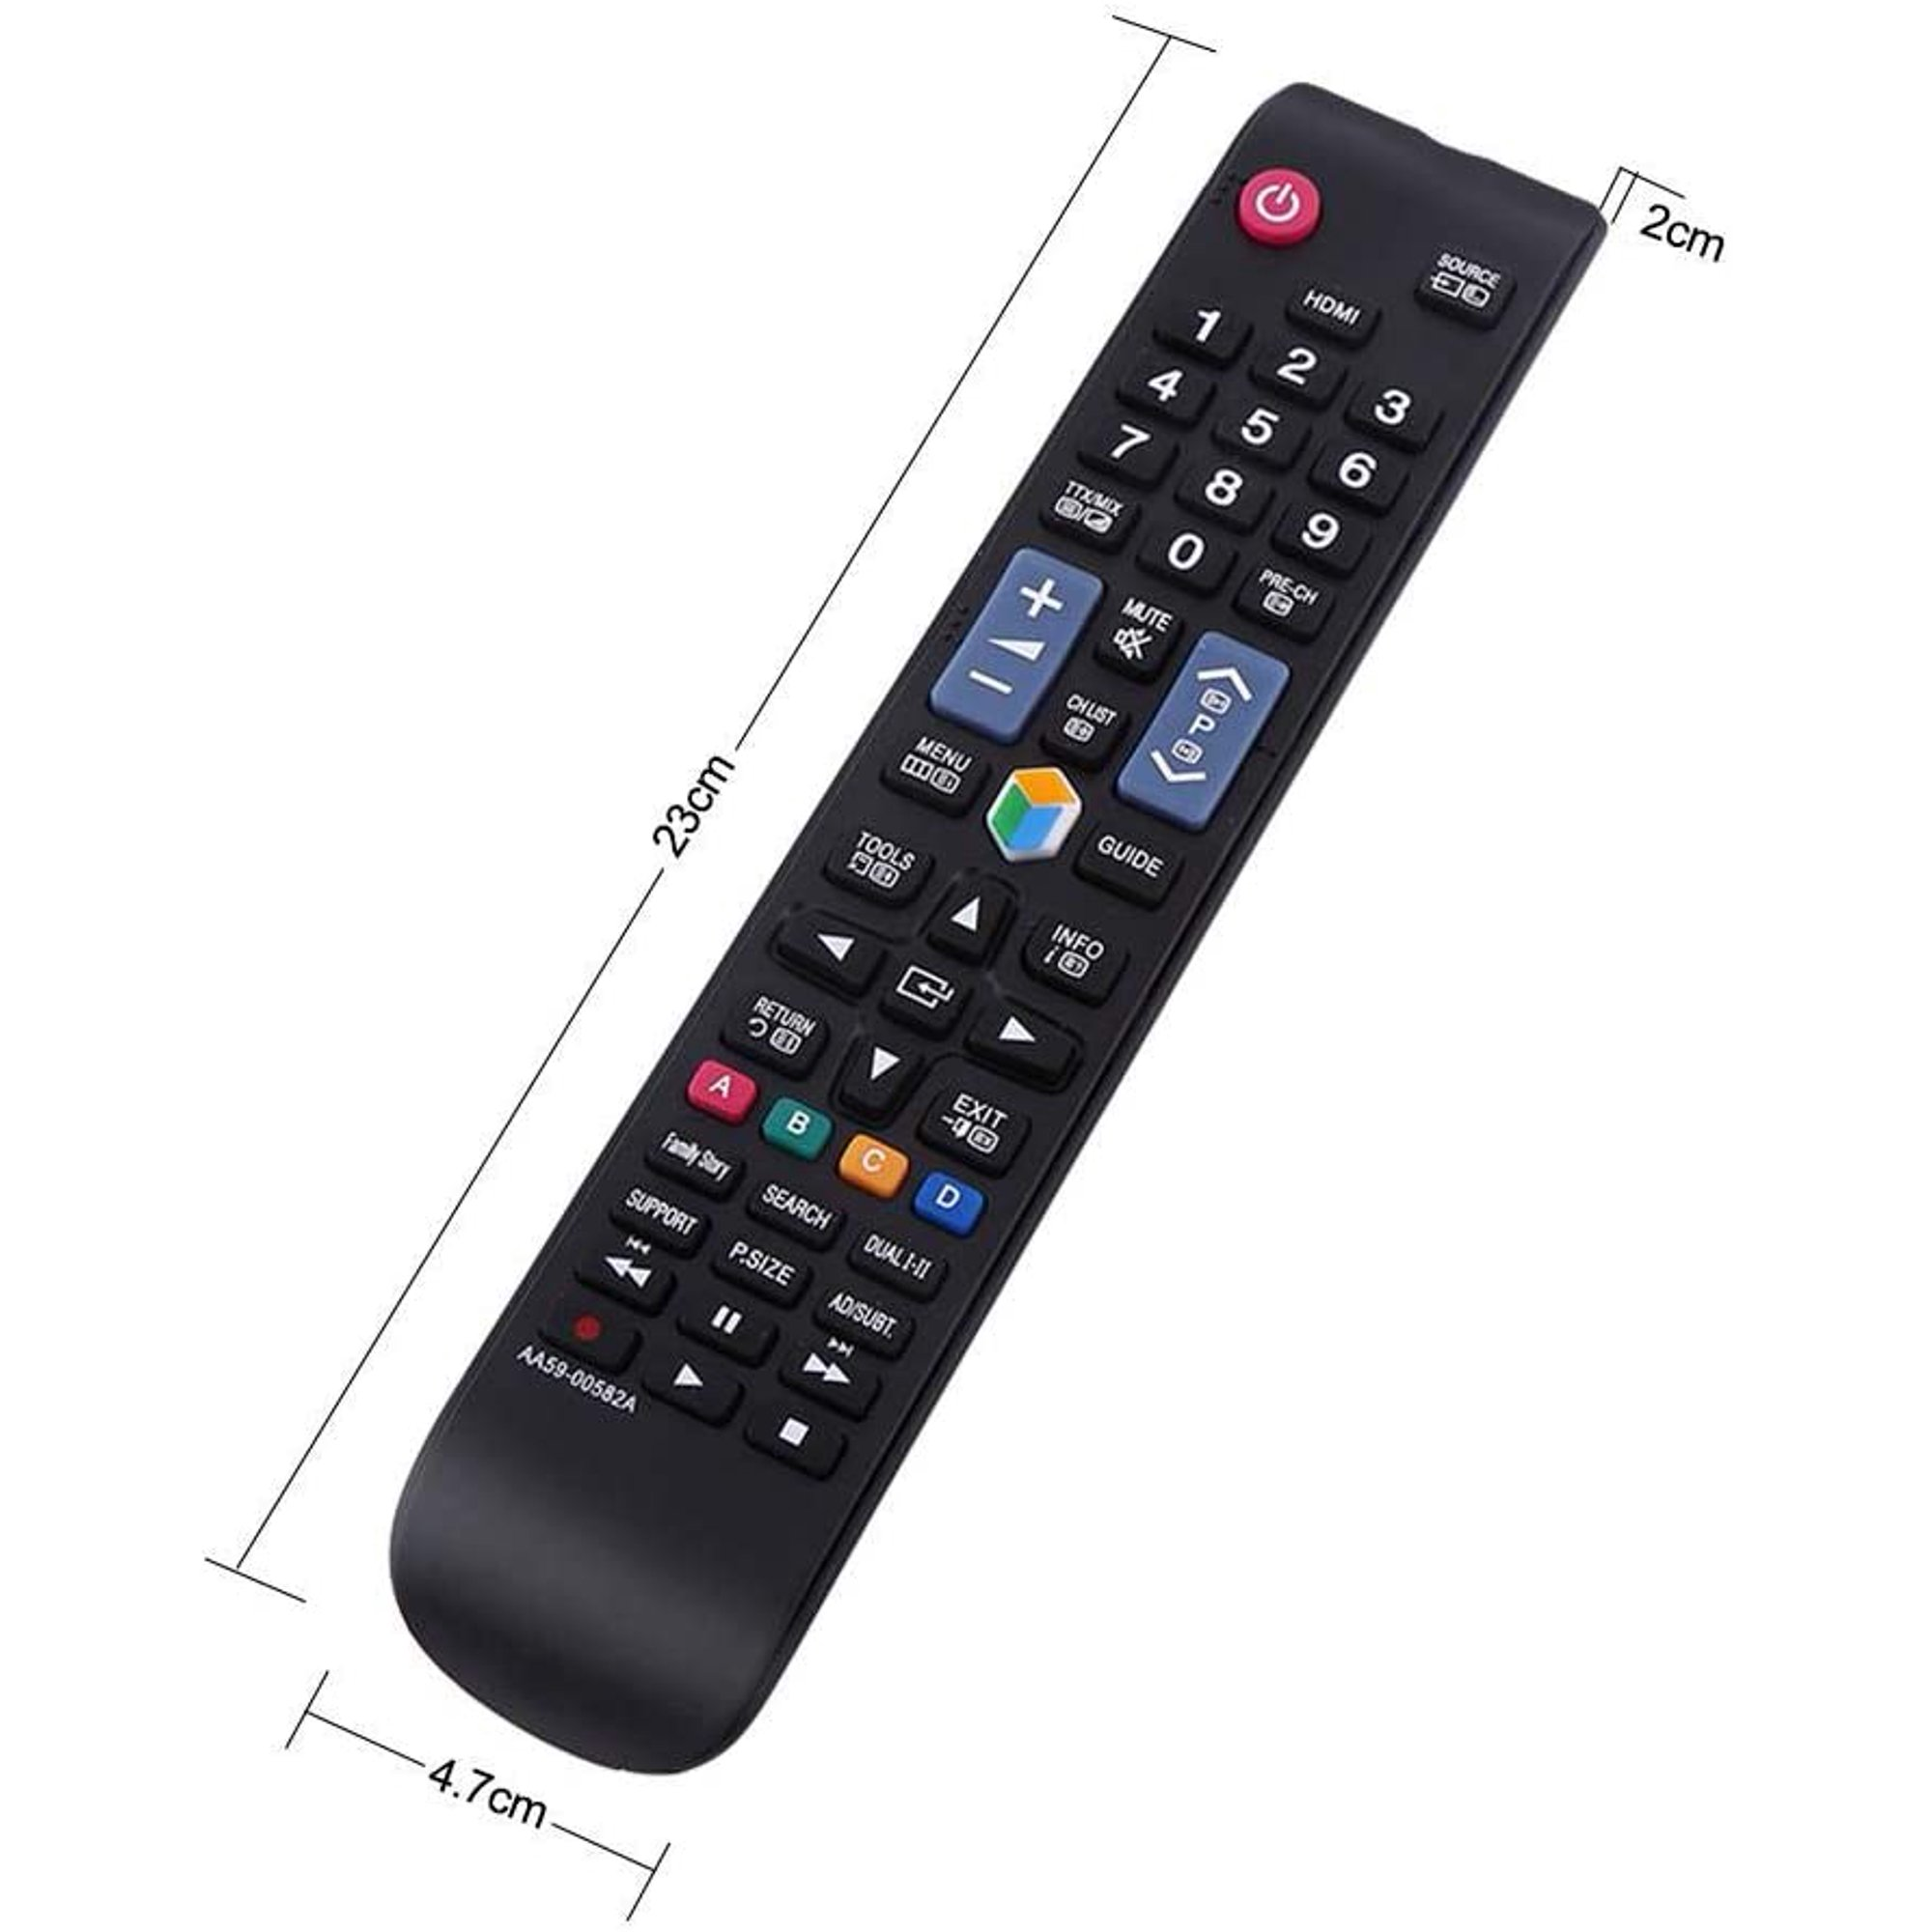
\includegraphics[width=8cm]{remote_controller}
    \caption{Samsung AA59-00584A}
\end{figure}

After several timing trials, I observed that the implemented protocol conforms to the timings found online on the page cited in the references \cite{8Samsung}. 

For convenience, I report the picture of the timings here:

\begin{figure}[h]
    \centering
    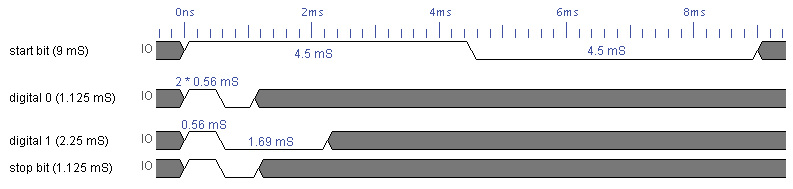
\includegraphics[width=15cm]{8_samsung}
    \caption{Samsung protocol timings}
\end{figure}

\newpage

\subsection{LCD 1602}
The LCD 1602\cite{lcd, i2cLcd} is an industrial character LCD that can display $16 \times 2$ or 32 characters at the same time, with a display font of $5 \times 8$ dots. The principle of the LCD 1602 liquid crystal display is to use the physical characteristics of the liquid crystal to control the display area by voltage,
that is, the graphic can be displayed.
\begin{figure}[h]
    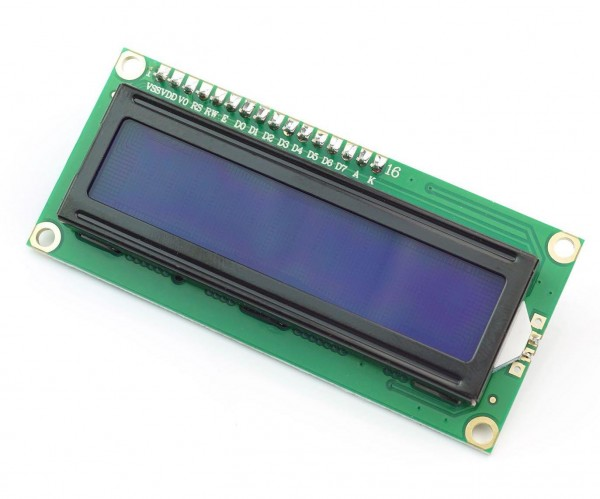
\includegraphics[width=7cm]{lcd}
    \centering
    \caption{LCD 1602}
\end{figure}

It is controlled through a parallel interface with:
\begin{itemize}
    \item 8-bit/4-bit data bus;
    \item 3 control signals.
\end{itemize}
The interface signals reach the two controller chips that drive the LCD panel:
\begin{figure}[h]
    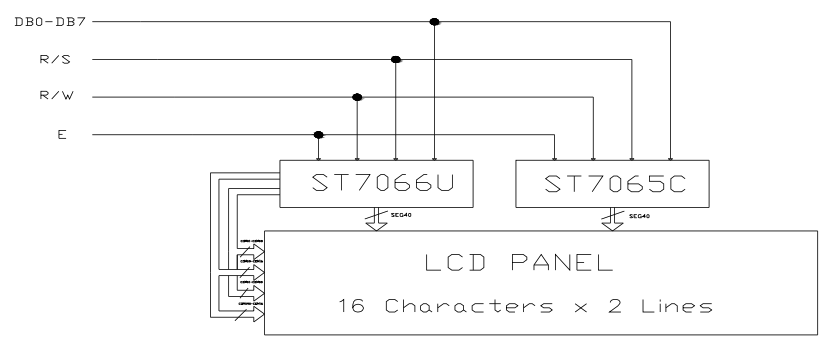
\includegraphics[width=14cm]{lcd_signals}
    \centering
    \caption{Block Diagram}
\end{figure}
\newpage
Pin assignments are summarized in this table:
\begin{figure}[h]
    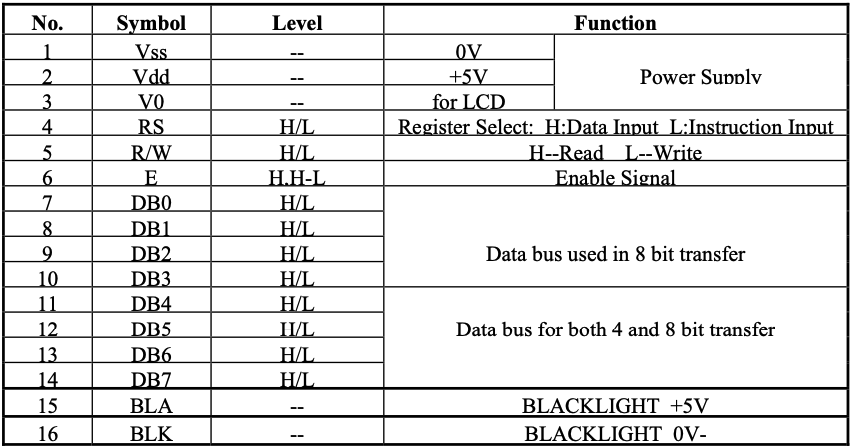
\includegraphics[width=13cm]{lcd_pin_assignments}
    \centering
    \caption{LCD pin assignments}
\end{figure}

To properly read or write data, some timing constraints must be observed. \\
Independently of whether we are reading or writing, the Enable signal must start its falling edge while DB$0$-DB$7$ are stable. If it is not, then erroneous data are sampled. 
The read or write mode is chosen only by the R/W signal, so only one case of these modes can be represented.
\begin{figure}[h]
    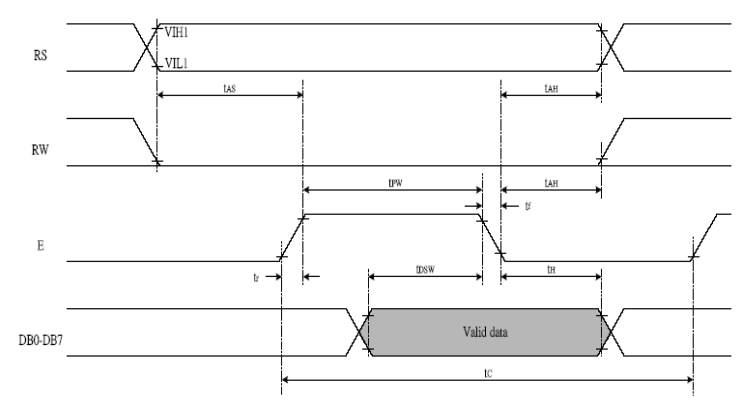
\includegraphics[width=12cm]{lcd_writing_data}
    \centering
    \caption{Writing timing characteristics}
\end{figure}

There are four categories of instructions that:
\begin{itemize}
    \item set display format, data length, cursor move direction, display shift etc.;
    \item set internal RAM addresses;
    \item perform data transfer from/to internal RAM;
    \item others.
\end{itemize}
A detailed description of how they can be realized is as follows:
\begin{figure}[h]
    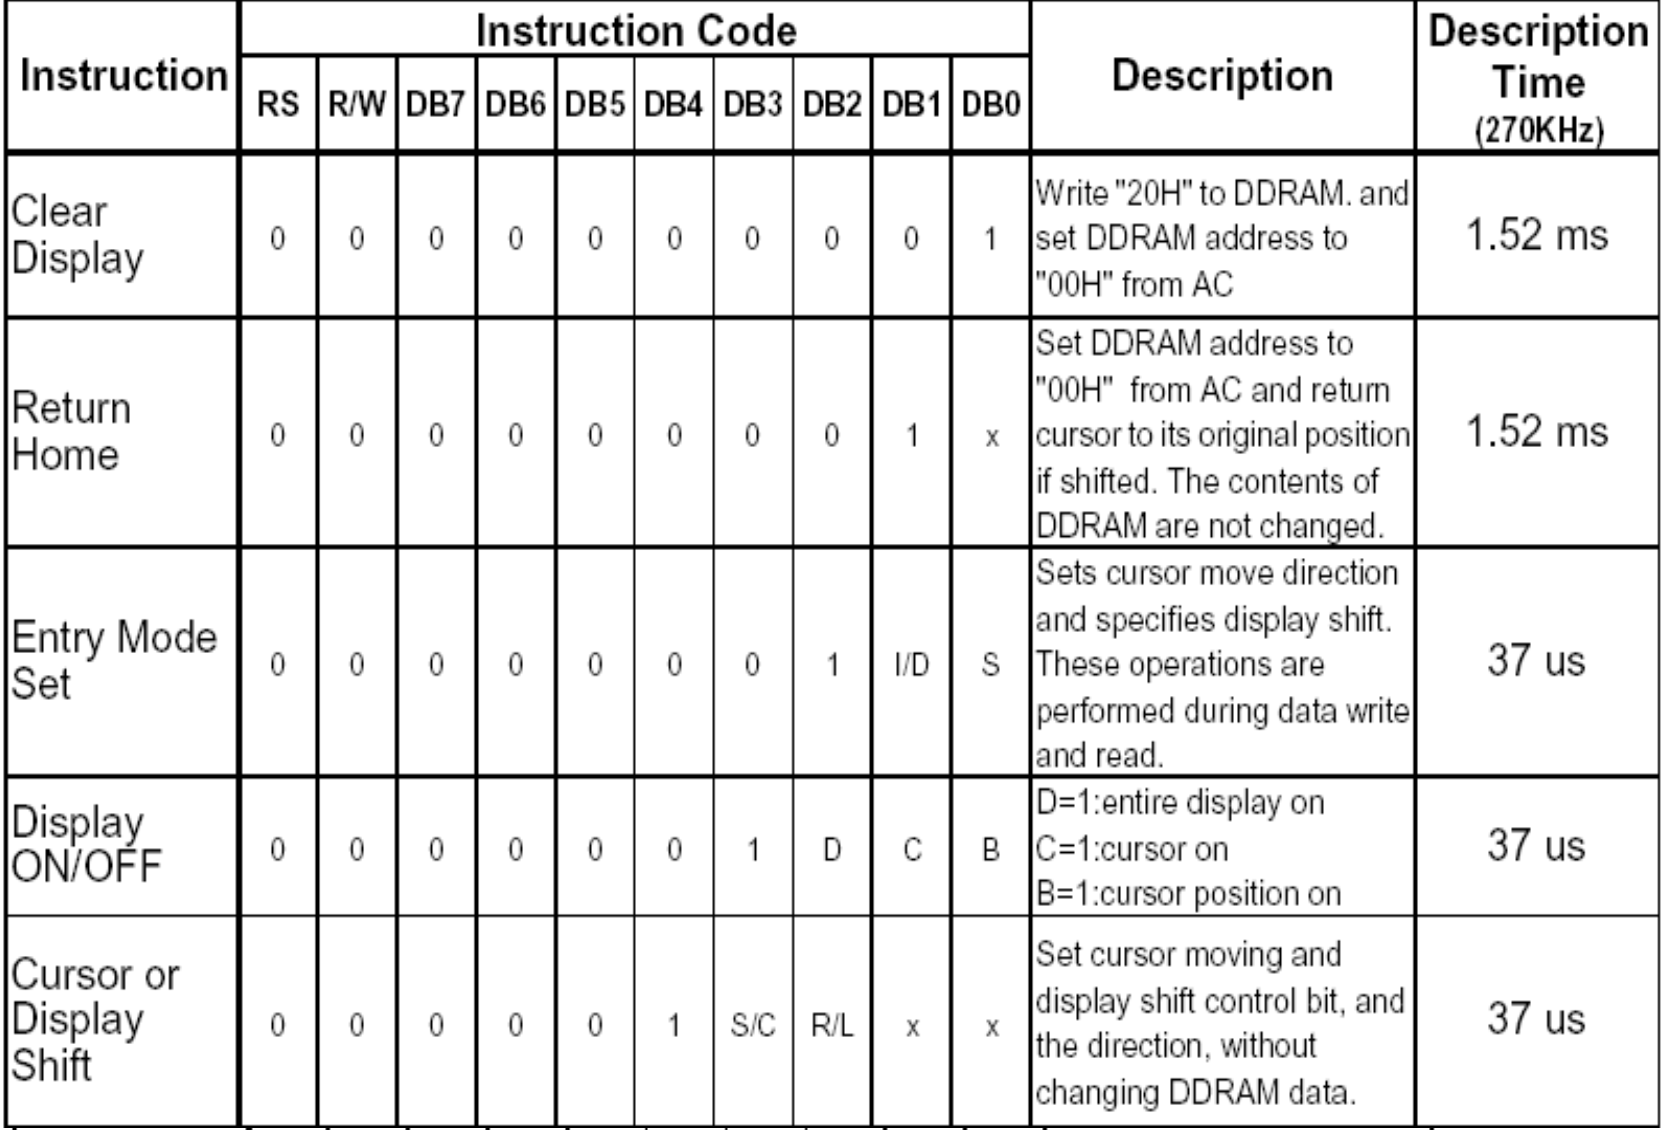
\includegraphics[width=11cm]{lcd_instructions_pt1}
    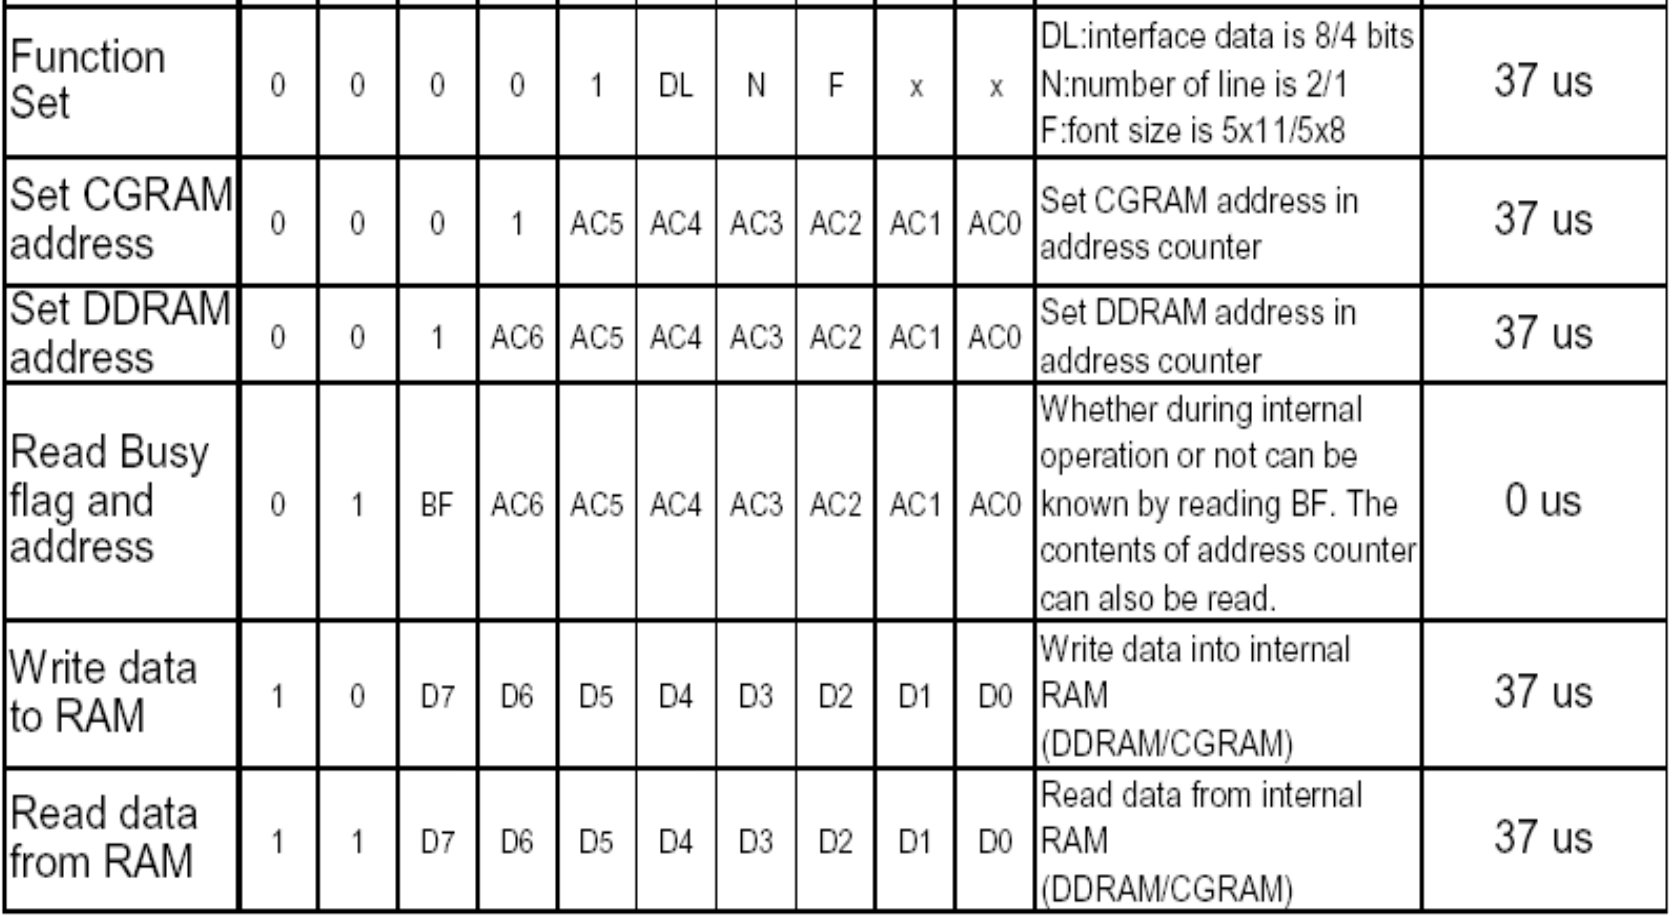
\includegraphics[width=11cm]{lcd_instructions_pt2}
    \centering
    \caption{Instruction Table}
\end{figure}

\subsection{IIC PCF8574AT Interface}
To ease the communication to the LCD display a serial I$^2$C module\cite{i2cLcd,PCF8574} has been used.
The interface connects its serial input and parallel output to the LCD, so only 4 lines can be used to do the job.

The I$^2$C bus was invented by Philips Semiconductor (now NXP Semiconductors). It can be described as:
\begin{itemize}
    \item synchronous;
    \item multi-master;
    \item multi-slave;
    \item packet switched;
    \item single-ended.
\end{itemize}

Each device connected to the bus is software-addressable by a unique address.

Two wires carry data (SDA - Serial DAta) and clock signals (SCL - Serial CLock), with the bus clock generated by the master.

It makes use of open-drain connections for bidirectional communication which allows us to transmit a logic low simply by activating a pull-down FET, which shorts the line to ground.
To transmit a logic high, the line is left floating, and the pull-up resistor pulls the voltage up to the voltage rail.

The PCF8574AT I/O expander for I$^2$C-bus contains:
\begin{itemize}
    \item 8-bit remote I/O pins (indicated as P0, P1, \dots, P7) used to transfer data;
    \item 3 address pins (indicated as A0, A1, A2) used to address the slave.
\end{itemize}

In this project, it is not necessary to read data from the I$^2$C LCD, so only the writing mechanism will be described.

\subsubsection{Writing mechanism}

To allow a master to send data to a slave device:
\begin{enumerate}
    \item the master, which acts as the transmitter, initiates communication by sending a START condition and addressing the slave, which acts as the receiver;
    \item the master sends data to the slave-receiver;
    \item the master terminates the transfer by sending a STOP condition.
\end{enumerate}

A high-to-low transition on the SDA line while the SCL is high is interpreted as a START condition. \\
In a reverse manner, a low-to-high transition on the SDA line while the SCL is high is interpreted as a STOP condition.

\begin{figure}[h]
    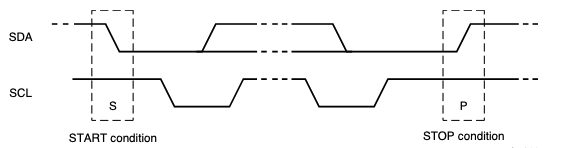
\includegraphics[width=11cm]{start_stop_conds}
    \centering
    \caption{START and STOP conditions}
\end{figure}

A sent byte can be a device address, a register address, or data written to a slave.

One data bit is transferred during each clock pulse. The data on the SDA line must remain stable during the HIGH period of the clock pulse as changes in the data line at this time will be interpreted as control signals. \\
Any number of data bytes can be transferred from the master to the slave between the START and STOP conditions. \\
Data is transferred starting from the MSB (Most Significant Bit).

After each byte of data has been transmitted, the master releases the SDA line to allow the slave-receiver to signal a successful transfer with an ACK (Acknowledge) or a failed transfer with a NACK (Not Acknowledge). \\
The receiver sends an ACK bit if the SDA is stable low during the high phase of the 9th period  of the clock. If the SDA line remains high, a NACK is sent.

\begin{figure}[h]
    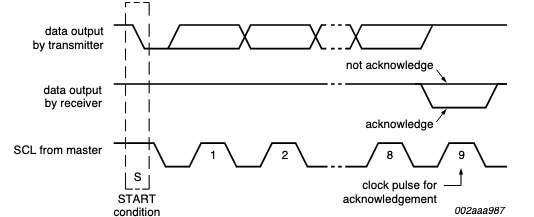
\includegraphics[width=11cm]{ACK_NACK}
    \centering
    \caption{Acknowledgements}
\end{figure}

Thus, there are 6 steps for the writing mechanism:
\begin{enumerate}
    \item the master sends the START condition and the slave address setting the
    last bit of the address byte to logic 0 for the write mode;
    \item the slave sends an ACK bit;
    \item the master sends the register address of the register it wishes to write to;
    \item the slave possibly acknowledges again;
    \item the master starts sending data;
    \item the master terminates the transmission with a STOP condition.
\end{enumerate}

\begin{figure}[h]
    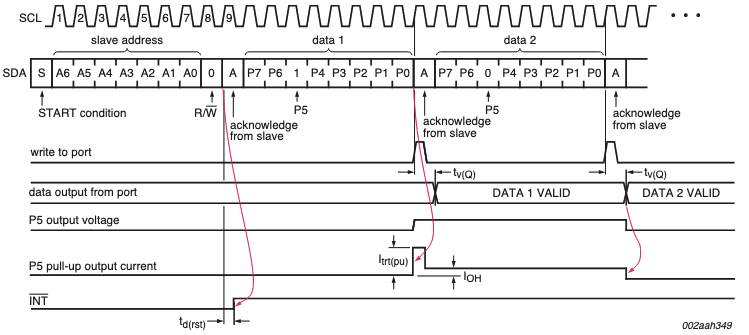
\includegraphics[width=14cm]{write_mode_expander}
    \centering
    \caption{Write mode (output)}
\end{figure}

All this work is done by the PCF8574AT interface.
All we need to do is to send the data byte for pins P7 to P0 after the slave address has been set correctly.

\subsubsection{PCF8574AT to LCD connection}
The PCF8574AT expander is soldered to the LCD pins according to the following scheme:

\begin{table}[h]
    \centering
    \begin{tabular}{c c} 
        \hline
        PCF8574AT pins & LCD pins \\ [0.5ex] 
        \hline\hline
        P0 & RS \\
        P1 & R/W \\
        P2 & E \\
        P3 & Backlight \\
        P4 & D4 \\
        P5 & D5 \\
        P6 & D6 \\
        P7 & D7 \\
        \hline
    \end{tabular}
    \caption{PCF8574AT to LCD pin connections}
\end{table}

Hence, the first time the LCD is turned on, it must be set to operate in 4 bit mode by sending the sequence:
\begin{table}[h]
    \centering
    \begin{tabular}{ | c | c | c | c | c | c | c | c | } 
        \hline
        D7 & D6 & D5 & D4 & Backlight & E & R/W & RS \\ [0.4ex] 
        \hline
        0 & 0 & 1 & 0 & 1 & 1 & 0 & 0 \\
        \hline
    \end{tabular}
    \\ [0.3cm] 
    \begin{tabular}{ | c | c | c | c | c | c | c | c | } 
        \hline
        D7 & D6 & D5 & D4 & Backlight & E & R/W & RS \\ [0.4ex] 
        \hline
        0 & 0 & 1 & 0 & 1 & 0 & 0 & 0 \\
        \hline
    \end{tabular}
    \caption{FUNCTION SET for 4 bit mode}
\end{table}

After this setting, instructions can be sent by transmitting the most significant nibble first. \\
As an example, suppose you want to display an E, whose ASCII code is 0x45. To accomplish this task, the sequence to be sent is as follows:
\begin{table}[h]
    \centering
    \begin{tabular}{ | c | c | c | c | c | c | c | c | } 
        \hline
        D7 & D6 & D5 & D4 & Backlight & E & R/W & RS \\ [0.4ex] 
        \hline
        0 & 1 & 0 & 0 & 1 & 1 & 0 & 1 \\
        \hline
        0 & 1 & 0 & 0 & 1 & 0 & 0 & 1 \\
        \hline
    \end{tabular}
    \\ [0.3cm] 
    \begin{tabular}{ | c | c | c | c | c | c | c | c | } 
        \hline
        D7 & D6 & D5 & D4 & Backlight & E & R/W & RS \\ [0.4ex] 
        \hline
        0 & 1 & 0 & 1 & 1 & 1 & 0 & 1 \\
        \hline
        0 & 1 & 0 & 1 & 1 & 0 & 0 & 1 \\
        \hline
    \end{tabular}
    \caption{Sending an ASCII E}
\end{table}

which means that the sequence to transmit is: 0x4D, 0x49, 0x5D, 0x59. \\
Command instructions are sent in the same way, except for the RS bit, which must be set to zero.

\subsection{Schematics}
All the hardware components shown in the previous sections have been connected with a breadboard to the Pi 4 as follows:
\begin{figure}[h]
    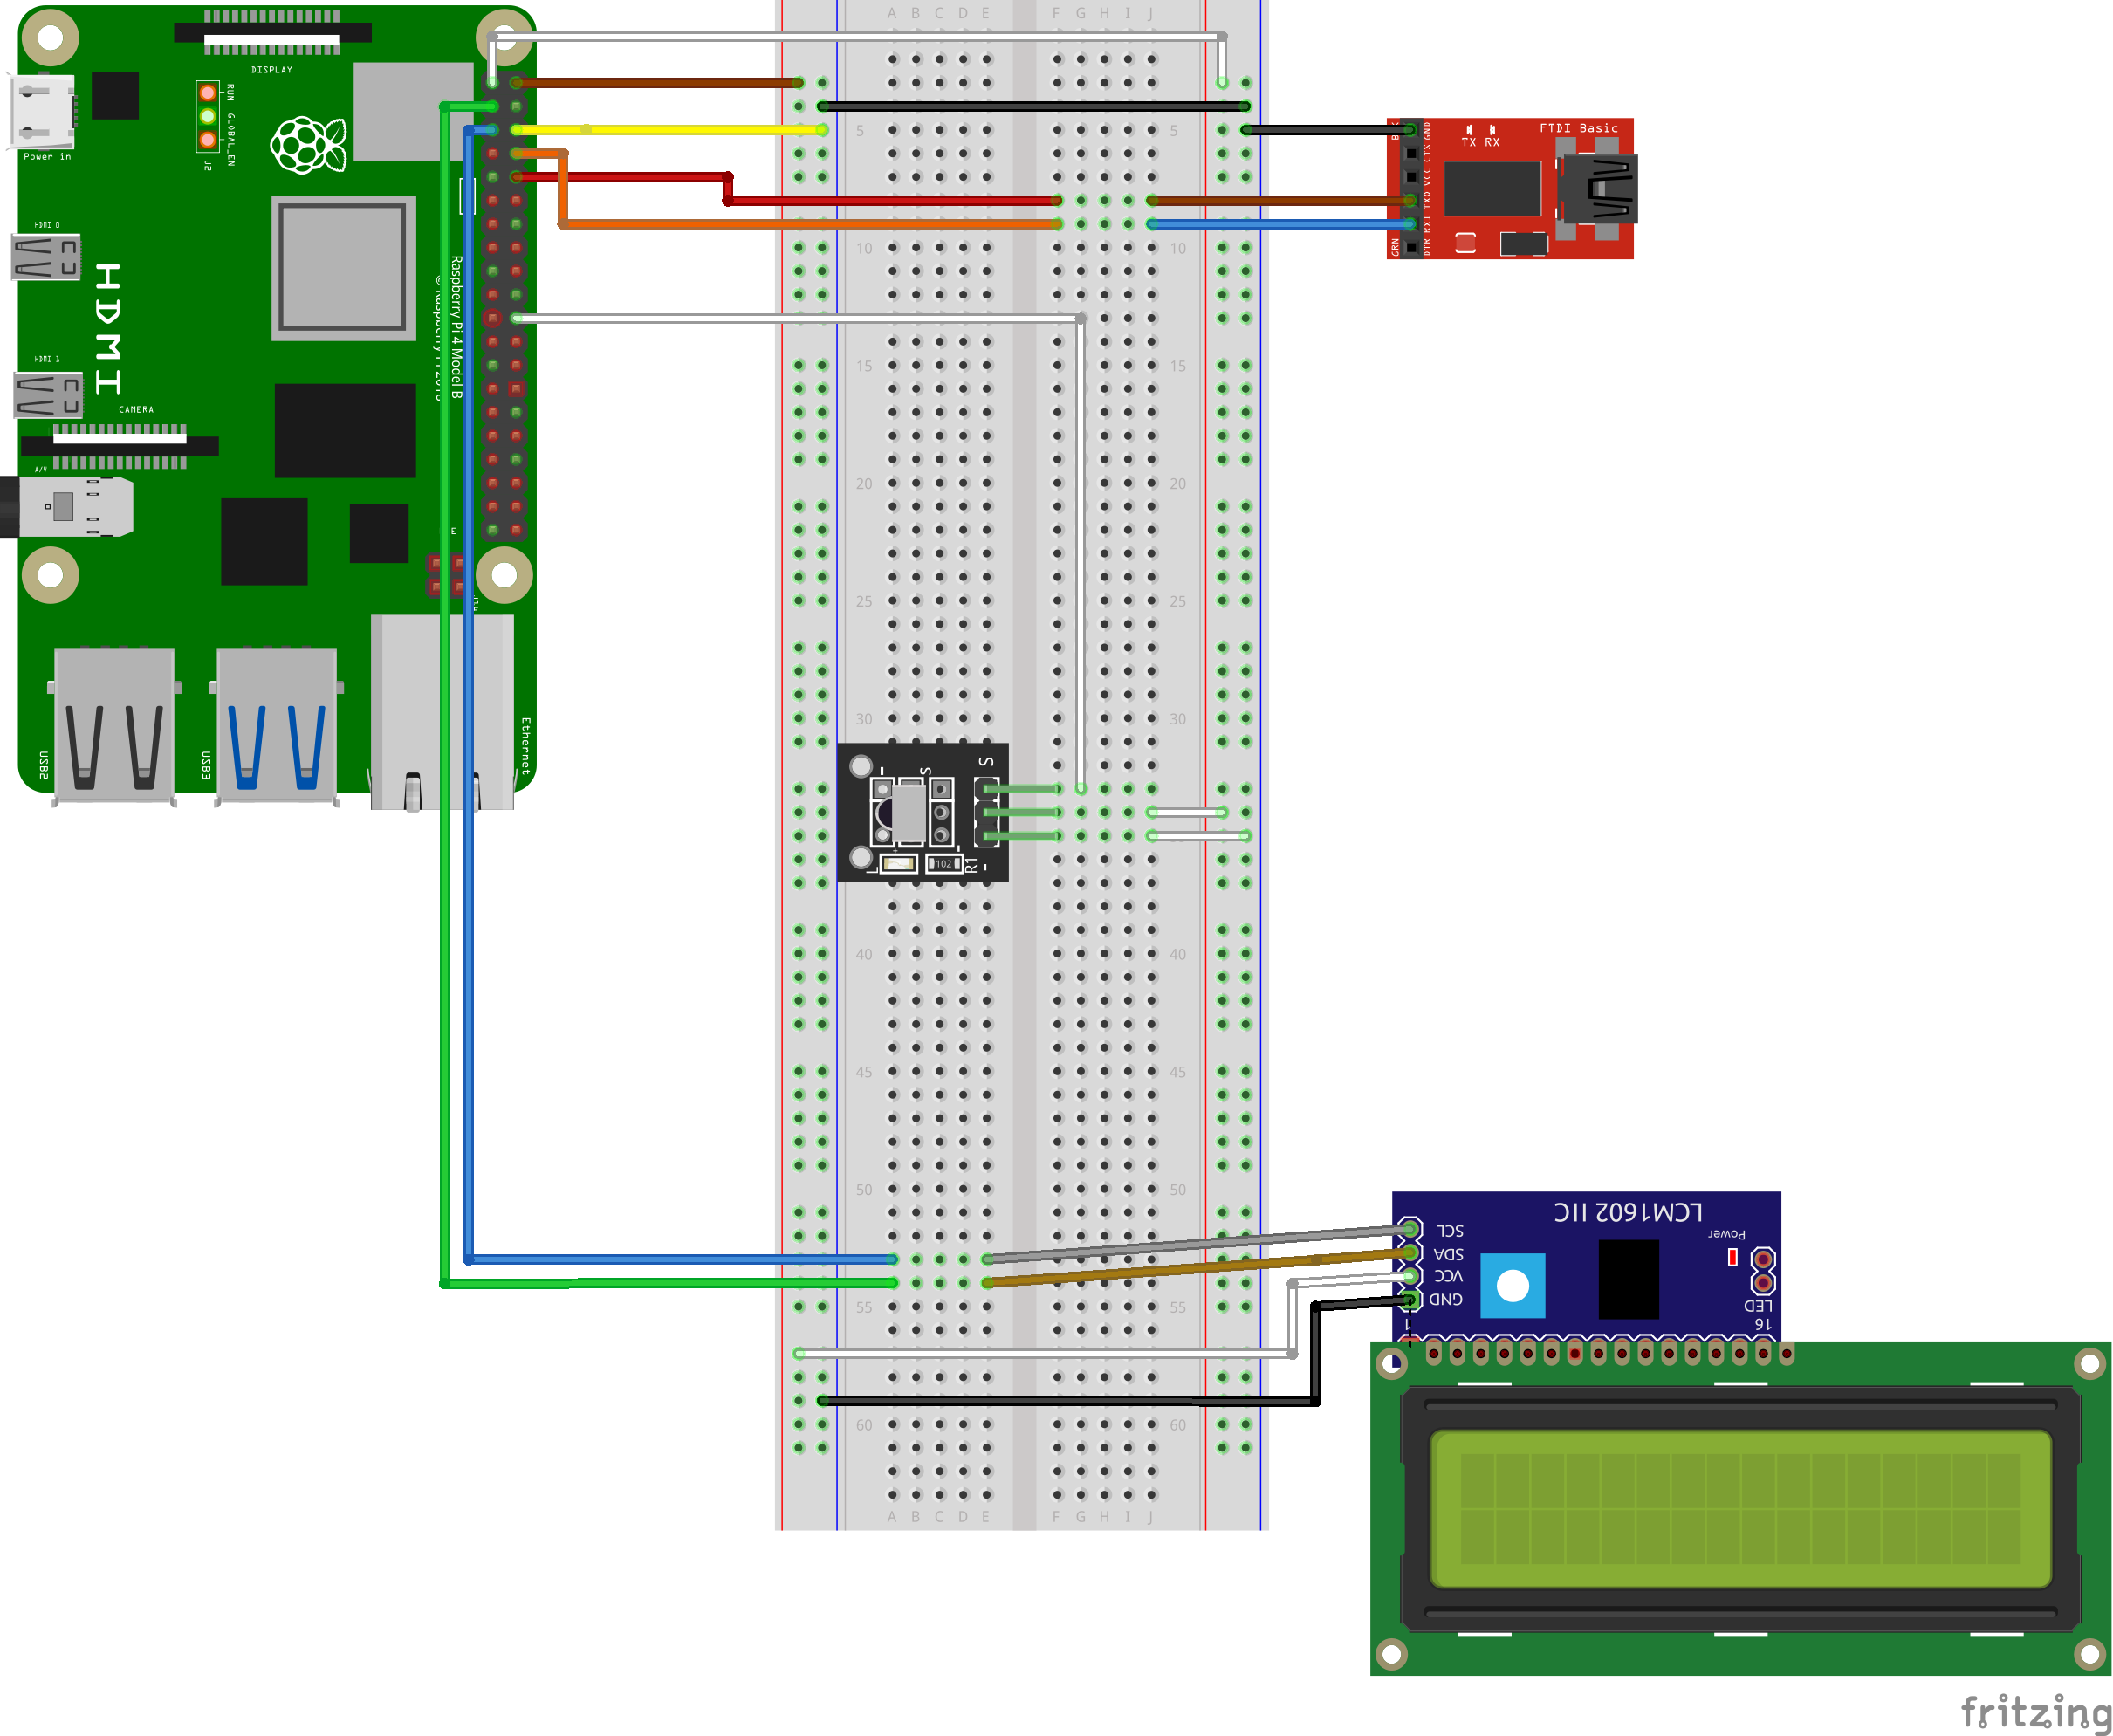
\includegraphics[width=14.3cm]{schematics}
    \centering
    \caption{Schematics}
\end{figure}

The following table summarizes all the connections between them and the Pi:
\begin{table}[h]
    \centering
    \begin{tabular}{c c c c} 
        \hline
        Pi 4 Model B & KY-022 & FT232RL & IIC PCF8574T \\ [0.5ex] 
        \hline\hline
        GPIO 25 & S & & \\
        3V3 power & +  & & \\
        GPIO 14 (TXD) & & RX  & \\
        GPIO 15 (RXD) & & TX  & \\
        5V power & & & VCC \\
        GPIO 2 (SDA) & & & SDA \\
        GPIO 3 (SCL) & & & SCL \\
        Ground & - & GND & GND \\
        \hline
        \end{tabular}
\end{table}

\section{Environment}

\subsection{pijFORTHos}
Forth is a programming language designed by \textit{Charles H. "Chuck" Moore} which can be implemented easily for resource-constrained machines due to its semplicity. \\
It is a procedural language heavely based on the use of the stack.

There are several dialects, each with its own definitions. The development involves the definition of new words, which added to the pre-existing vocabulary, can create the final application incrementally and naturally.

pijFORTHos\cite{pijFORTHos} is a bare-metal FORTH interpreter for the Raspberry Pi, based on Jonesforth-ARM\cite{JonesforthARM}. 

Jonesforth-ARM is an ARM port of x86 JonesForth, which is a Linux-hosted FORTH presented in a Literate Programming style by \textit{Richard W.M. Jones}.

pijFORTHos represents the base on which the application is built.

\subsection{Minicom and Picocom}
\textbf{Minicom}\cite{minicom} is a terminal emulation program for Unix-like operating systems, used for communication and typically to set up a remote serial console.

\textbf{Picocom}\cite{picocom} is, in principle, very much like minicom. It was designed to serve as a simple, manual, modem configuration, testing, and debugging tool.

\textbf{ASCII-XFR}\cite{ASCIIXFR} transfers files in ASCII mode. It is used to send the source file to the Raspberry because it
allows a delay between each character and line sent. \\
Given that the UART is asynchronous, this is a needed feature because it avoids overrun errors and lost characters if the receiver is busy while executing or compiing FORTH words.

Picocom is launched on the development machine through the command:
\begin{Verbatim}[breaklines=true, breakanywhere=true]
    picocom --b 115200 /dev/cu.usbserial-A50285BI --send "ascii-xfr -sv -l100 -c10" --imap delbs
\end{Verbatim}

It is launched with the same VCP (Virtual COM Port) parameters as the Pi UART:
\begin{itemize}
    \item \texttt{--b 115200}: 115200 bit/s bit rate;
    \item \texttt{/dev/cu.usbserial-A50285BI}: the serial UART device;
    \item \texttt{--send "ascii-xfr -sv -l100 -c10"}:
    
    specifies ascii-xfr as the external
    command to use for transmitting files. \\
    The options used are: 
    \begin{itemize}
        \item \texttt{-sv}: verbose send mode;
        \item \texttt{-l100}: sets a 100 milliseconds delay after each line is sent,
        this usually gives enough time to run a command and be
        ready for the next line in time;
        \item \texttt{-c10}: waits 10 milliseconds between each character sent.
    \end{itemize}
    \item \texttt{--imap delbs}: allows the use of backspace to delete a character.
\end{itemize}

\subsection{Script}
Since the serial UART has a limited operating speed, one way to speed up the loading of the entire project is to delete all comments and merge the files into a single file.

As not everyone has a Unix-like operating system, the first part of the script (\texttt{create\_program.sh}) is made for Zsh, but can be easily changed to other shells because it simply prints the files to the stdout. 

\lstinputlisting[language=sh]{../create_program.sh}

The second part (\texttt{unify\_and\_uncomment.py}) is done in Python, because today almost everyone has a Python interpreter in their system. It reads from stdin, deleting comments and joining all words by separating them with a single space.

\lstinputlisting[language=python, breaklines=true]{../unify_and_uncomment.py}

Script files must have execution permissions to run. If you are using a Unix-like operating system you can grant them by typing in a terminal window (assuming you are in the project folder):

\begin{Verbatim}[breaklines=true, breakanywhere=true]
    chmod u+x unify_and_uncomment.py
    chmod u+x create_program.sh
\end{Verbatim}

and then build the project by simply writing (assuming that you have changed the shell and python interpreter):

\begin{Verbatim}[breaklines=true, breakanywhere=true]
    ./create_program.sh
\end{Verbatim}
\section{Software}

\subsection{Prerequisites}

The files needed to be placed in the micro SD card to run the software are as follows:
\begin{itemize}
    \item \texttt{bootcode.bin};
    \item \texttt{config.txt};
    \item \texttt{fixup.dat};
    \item \texttt{start4.elf};
    \item \texttt{kernel7.img} (which contains pijFORTHos);
    \item \texttt{bcm2711-rpi-4-b.dtb}.
\end{itemize}

An empty micro SD card with only those files is sufficient. \\ 
If you do not have these files, you can download them from the official repository\footnote{\url{https://github.com/raspberrypi/firmware}} or operate in this way: you can format the micro SD card for the Pi 4 using the official software called Raspberry Pi Imager\footnote{\url{https://www.raspberrypi.com/software/}}, released by Raspberry Pi. \\
When you open the program, you are asked to choose an operating system. You can select Raspberry Pi OS (32 bit) and continue with formatting.

Once the formatting is complete\footnote{Please read the following subsection first to avoid repeating the procedure}, you need to remove the \texttt{kernel*.img} and insert the \texttt{kernel7.img} that contains pijFORTHos.

Your \texttt{config.txt} file must contain the following uncommented options:

\begin{Verbatim}[breaklines=true, breakanywhere=true]
    dtparam=i2c_arm=on
    enable_uart=1
\end{Verbatim}

which enable the I$^2$C and the UART, respectively.

\subsubsection{How to get IIC LCD slave address}

For the project to work, it is important to know the correct slave address.

A visual method to recognize the address is to analyze the expander structure as follows\cite{i2cLcd}:
\begin{figure}[h]
    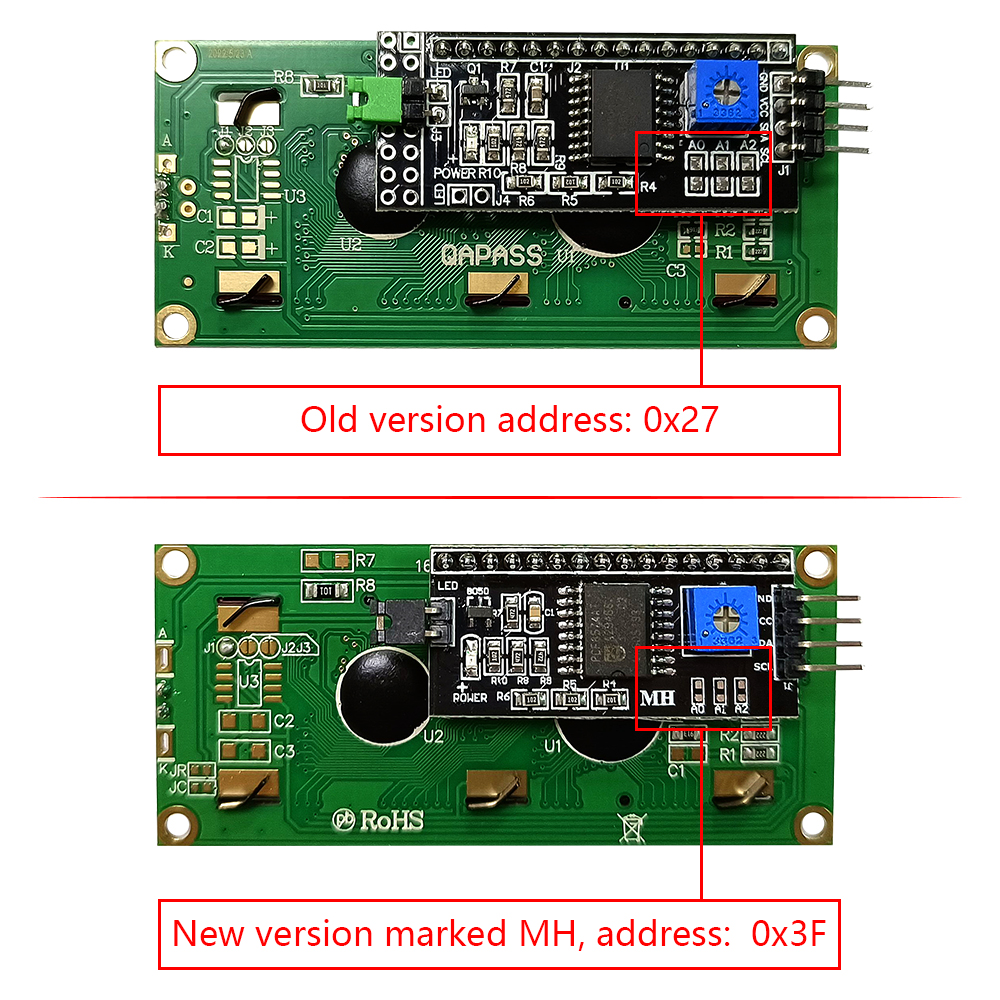
\includegraphics[width=14cm]{i2c_lcd}
    \centering
    \caption{PCF8574AT I/O expander}
\end{figure}

If it doesn't work and you still can't figure out what the address is you can operate using Raspbian. \\
Open a terminal window and install \texttt{i2c-tools}:
\begin{Verbatim}[breaklines=true, breakanywhere=true]
    sudo apt-get install i2c-tools
\end{Verbatim}

Once the download is complete, you can simply type:
\begin{Verbatim}[breaklines=true, breakanywhere=true]
    i2cdetect -y 1 
\end{Verbatim}
Now, if the connection on the breadboard is correct, you should see the slave address in the center of the array. \\
In my case, the I$^2$C slave address is 0x27.

\subsubsection{How to run}

Once you have downloaded the project, you can port it to \textbf{Raspberry Pi 3 Model B} and \textbf{Raspberry Pi 3 Model B+} by changing the \texttt{PERI\_BASE} constant to \texttt{0x3F000000} (\texttt{utils.f})\footnote{For the project to work, the boot files must also be changed}. \\
After possibly performing this operation and reading the previous subsection, having changed if necessary the literal used to set the slave address into the word \texttt{INIT\_I2C} (\texttt{i2c.f}), you can run the script and load the program as follows:
\begin{enumerate}
    \item execute \texttt{./create\_program.sh} and run 
        \begin{Verbatim}[breaklines=true, breakanywhere=true]
        picocom --b 115200 /dev/cu.usbserial-A50285BI --send "ascii-xfr -sv -l100 -c10" --imap delbs
        \end{Verbatim}
    \item load the file \texttt{program.f} generated by the script using \keys{\ctrl + A} and \keys{\ctrl + S}, and writing the path to the file, e.g. \texttt{./program.f};
    \item start the program by typing \texttt{MAIN} and pressing \keys{\return}.
\end{enumerate}

\subsection{Code structure}

The project is composed of 9 files:
\begin{itemize}
    \item \texttt{jonesforth.f};
    \item \texttt{se-ans.f};
    \item \texttt{utils.f};
    \item \texttt{timer.f};
    \item \texttt{i2c.f};
    \item \texttt{lcd.f};
    \item \texttt{ir\_receiver.f};
    \item \texttt{lookup\_table.f};
    \item \texttt{main.f};
\end{itemize}

The development process followed a bottom-up methodology, so the files are listed in an ascending order of abstraction.

Each file consists of a module, which contains all the constants and words necessary for the proper functioning of that module.

Given the information on the previous pages, it should be clear how the project works. In addition to the defined words, there are comments explaining what may not be perfectly clear.

\subsubsection{ANSI Compliance}
JonesForth does not conform to ANSI\cite{ANSICompliance} standards, which means that some words do not behave as expected.

For this reason, the first file \texttt{jonesforth.f}, which contains words such as \texttt{S"}, is loaded as the first file, to ensure that \texttt{OF} and \texttt{ENDOF} used in \texttt{lookup\_table.f} can function properly.

After this necessary operation, regardless of the files containing the above words, all subsequent words are ANSI-compliant thanks to the file \texttt{se-ans.f}, created by Professor Daniele Peri.

\subsubsection{jonesforth.f}
\VerbatimInput[fontsize=\footnotesize, breaklines=true, breakanywhere=true]{../jonesforth.f}

\subsubsection{se-ans.f}
\VerbatimInput[fontsize=\footnotesize, breaklines=true, breakanywhere=true]{../se-ans.f}

\subsubsection{utils.f}
\VerbatimInput[fontsize=\footnotesize, breaklines=true, breakanywhere=true]{../utils.f}

\subsubsection{timer.f}
\VerbatimInput[fontsize=\footnotesize, breaklines=true, breakanywhere=true]{../timer.f}

\subsubsection{i2c.f}
\VerbatimInput[fontsize=\footnotesize, breaklines=true, breakanywhere=true]{../i2c.f}

\subsubsection{lcd.f}
\VerbatimInput[fontsize=\footnotesize, breaklines=true, breakanywhere=true]{../lcd.f}

\subsubsection{ir\_receiver.f}
\VerbatimInput[fontsize=\footnotesize, breaklines=true, breakanywhere=true]{../ir_receiver.f}

\subsubsection{lookup\_table.f}
\VerbatimInput[fontsize=\footnotesize, breaklines=true, breakanywhere=true]{../lookup_table.f}

\subsubsection{main.f}
\VerbatimInput[fontsize=\footnotesize, breaklines=true, breakanywhere=true]{../main.f}

\subsection{Possible improvements}

The project could be extended to respond to IR signals, that is, to store the last sampled command and, through the use of a simple button (e.g. DAOKAI 4Pin button), decide when to send it to the TV using an IR transmitter (e.g. KY-005). \\
In this way, the button acts as a trigger and the application is able to send and receive signals.

\begin{figure}[ht]
    \centering
    \subfigure[KY-005]{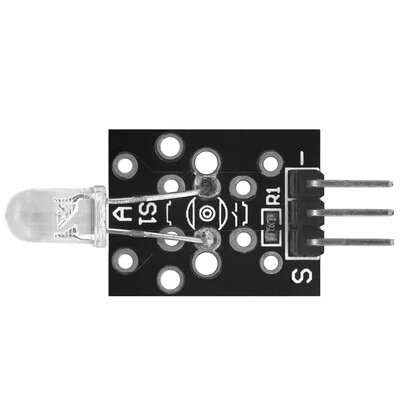
\includegraphics[width=5cm]{ir_transmitter}} 
    \subfigure[DAOKAI 4Pin button]{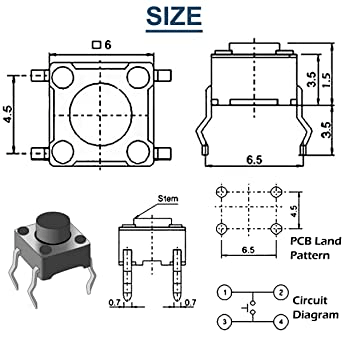
\includegraphics[width=5cm]{button.png}} 
    \caption{Additional hardware}
\end{figure}

In addition to this improvement, one might consider using the Pi 4's green ACT LED to communicate with the user, for example, to signal that a command has been processed correctly or that something has gone wrong.

\printbibliography
\end{document}